\chapter{Comportamientos} \label{cap:comportamientos}
% BREVE DESCRIPCIÓN DEL CONTENIDO DE ESTE CAPÍTULO
En este capítulo se definirán y diseñarán los comportamientos que necesita el vehículo no tripulado para realizar una conducción autónoma. Al comenzar, en la sección \ref{sec:introducción_a_comportamientos} se da una introducción para los comportamientos esperados del vehículo, enseguida la sección \ref{sec:paradigmas_de_la_robótica} expone los diferentes paradigmas de la robótica y específica que paradigma implementará el robot (vehículo). A continuación, en la sección \ref{sec:comportamientos_del_vehículo} se definen tres comportamientos que el vehículo debe realizar, las subsecciones \ref{sub:crucero}, \ref{sub:mantener_distancia} y \ref{sub:rebase} de esta sección responden a las preguntas de ¿Qué?, ¿Cómo? y ¿Cuándo? se realiza cada comportamiento. Finalmente, la subsección \ref{sub:árbitro} explica el sistema de decisión que controla los comportamientos.

Para este capítulo las implementaciones en código de los comportamientos así como algún cambio en las leyes de control previamente establecidas son con el lenguaje de programación Python.

\section{Introducción a comportamientos} \label{sec:introducción_a_comportamientos}

Tal como se explicó en la sección \ref{sub:niveles_de_autonomía} de capítulo \ref{cap:antecedentes}, un conductor requiere de diferentes habilidades para realizar funciones tácticas y operativas durante el acto de conducir. También, se mencionó que un vehículo autónomo no cuenta de manera natural con estas habilidades, pero si tiene distintos sensores y algoritmos que le ayudan a percibir y conocer el ambiente donde se encuentra. La respuesta o conjunto de respuestas que puede presentar un vehículo no tripulado en situaciones de viales se conoce como comportamiento, la forma en que el robot (vehículo) utiliza las herramientas con las que cuenta son clave para definir uno o varios comportamientos. Al igual que un conductor humano, el vehículo autónomo debe responder correctamente ante diferentes situaciones vehiculares, por ejemplo; mantener una ruta, realizar un rebase, frenar repentinamente o incluso controlar cuidadosamente la velocidad y distancia en situaciones de tráfico.

En este trabajo se pretenden desarrollar tres comportamientos que ayuden al vehículo de pruebas a completar la DDT (\textit{Dynamic Driving Task}) para navegación autónoma con situaciones y condiciones cercanas a la realidad, estos comportamientos son:
\begin{enumerate}
    \item \textbf{Crucero:} Para navegación autónoma sin obstáculos.
    \item \textbf{Rebase:} Para navegación autónoma con obstáculos.
    \item \textbf{Mantener Distancia:} Para navegación en situación de tráfico.
\end{enumerate}
Retomando los conceptos de funciones tácticas y operativas descritas en el capítulo \ref{cap:antecedentes}, el vehículo puede y debe cambiar de comportamiento según las condiciones actuales, para ello es necesario contar con un sistema de decisión que haga el cambio entre comportamientos. En secciones posteriores se describirán estos tres comportamientos además de un árbitro encargado para la toma de decisiones.

\section{Paradigmas de la robótica} \label{sec:paradigmas_de_la_robótica}

Una filosofía o conjunto de suposiciones y técnicas que caracterizan un enfoque para una clase de problemas en particular se conoce como paradigma. Un paradigma es además, una forma de ver el mundo como un conjunto implícito de herramientas en la resolución de problemas. Con este concepto, algunos problemas parecen más adecuados para diferentes enfoques. Por lo tanto, ningún paradigma es del todo correcto y mucho menos absoluto, simplemente tienen procesos diferentes \cite{murphy2019introduction}.

%Por ejemplo, existen problemas matemáticos que podrían resolverse en un sistema cartesiano con coordenadas $(x, y, z)$, pero en ocasiones resulta más sencillo resolver el mismo problema mediante el uso de coordenadas polares $(r, \theta)$. En el campo del cálculo, las coordenadas cartesianas y polares representan dos paradigmas diferentes para manipular un problema. Ambos producen respuestas similares y correctas. Sin embargo, alguno de estos paradigmas puede requerir un menor esfuerzo respecto al otro para el mismo problema.

Un ejemplo de esto son los paradigmas de la programación. Cualquier solución a un problema que pueda ser expresada en forma de algoritmo pude ser implementada mediante algún lenguaje de programación y posteriormente ser procesada por una computadora. En programación existen diferentes paradigmas de programación como: imperativo, declarativo, orientado a objetos, reactivo, entre otros. Cada uno de estos paradigmas posee características propias y están diseñados para implementar soluciones a cuestiones particulares. Problemas lógico-matemáticos sencillos pueden ser resueltos mediante cualquiera de estos paradigmas, pues todos permiten alcanzar una solución correcta y la diferencia radica en la cantidad de esfuerzo que requiere cada paradigma.

El ecosistema de la robótica recupera esta misma idea de paradigma. Aplicar el paradigma correcto permite facilitar la resolución de problemas. Por lo tanto, conocer los paradigmas de la robótica e inteligencia artificial es clave para programar con éxito un robot y lograr una meta particular. En la actualidad existen tres paradigmas en robótica: Jerárquico, Reactivo e Híbrido (Deliberativo - Reactivo). Los paradigmas de la robótica se describen de dos maneras diferentes.

\begin{enumerate}
    \item Por la relación que existe entre las tres primitivas de la robótica: Sentir, Planear y Actuar. Por ejemplo, si una función del robot percibe información de los sensores que lo instrumentan y produce una salida útil para otras funciones, entonces esa función entra en la clasificación de Sentido. Si la función está recibiendo información y produce una o más tareas por realizar (avanzar 2 metros, girar a la izquierda y detenerse) se trata de una función en la categoría de Plan. Finalmente, las funciones que producen comandos de salida hacia los actuadores del robot caen dentro de la categoría de Actuar (girar $n$ grados en sentido horario, con velocidad angular $\omega$).
    
    \item Por la forma en que la información de los sensores es procesada y distribuida a través del sistema. En algunos paradigmas la información de los sensores está restringida para ser utilizada de forma especial en cada función del robot. Otros paradigmas esperan que toda la información del o los sensores primero sea procesada por un modelo global y después los subconjuntos del modelo se distribuyan a otras funciones conforme sea necesario.
\end{enumerate}

\subsection{Paradigma jerárquico} \label{sub:paradigma_jerárquico}

El paradigma jerárquico es el método históricamente más antiguo para organizar inteligencia robótica tradicional. Prevaleció fuertemente desde el año de 1967, con la aparición del primer robot con IA, Shakey\cite{kuipers2017shakey}, hasta principios de la década de 1990. Este paradigma funciona de manera descendente, es decir, de arriba hacia abajo y con mucha planificación. Se basa en una visión introspectiva de como piensan los humanos.``Veo una silla, decido sentarme en ella y genero una trayectoria hacia ella evitando obstáculos". Un robot que implementa el paradigma jerárquico, percibe el mundo, planifica la siguiente acción y después actúa (Sensa, Planea y Actúa), ver \ref{fig:hierarchical_paradigm}. Dicho de otro modo, este paradigma es secuencial y ordenado. En cada paso el robot planifica explícitamente el movimiento siguiente. Otra característica fundamental del modelo jerárquico es que toda la información percibida por los sensores tiende a reunirse en un modelo global o una sola representación que el sistema planificador (Planear) utiliza para encaminarse a realizar acciones (Actuar) \cite{murphy2019introduction}. 
%El proceso de ejecución de cada paso en el paradigma jerárquico es: Primero, el robot detecta el mundo y construye un mapa global de este. Después, con los ojos cerrados, planifica todas las acciones necesarias para alcanzar la meta. Posteriormente, el robot actúa para llevar a cabo la primer acción. Al final, cuando el robot ha llevado a cabo la secuencia Sentir-Planear-Actuar \ref{fig:hierarchical_paradigm}, comienza nuevamente el ciclo de manera iterativa.
La detección o el efecto de sentir en el paradigma jerárquico es de manera monolítica: todas las observaciones de los sensores se fusionan en una estructura de datos global , a la que puede acceder el planificador. Esta estructura de datos se conoce como modelo de mundo, donde el término mundo hace referencia tanto al mundo exterior como cualquier otro significado que el robot le atribuya. Dentro de este paradigma el modelo de mundo contiene típicamente:
\begin{enumerate}
    \item Una representación \textit{a priori} del entorno en que el robot opera.
    \item Información de detección del ambiente.
    \item Cualquier conocimiento cognitivo adicional que resulte necesario para realizar una tarea.
\end{enumerate}

El paradigma Jerárquico ofrece diferentes ventajas como: orden en la relación Sensar-Planear-Actuar, fomentar la programación monolítica y funcional. Sin embargo, al ser el más antiguo cuenta con varias desventajas entre las que destacan: lenta ejecución en algoritmos de detección y planificación, Requiere la mayor cantidad de información posible del entorno, además de no toma en cuenta la incertidumbre en sensores y actuadores.

\begin{figure}
    \centering
    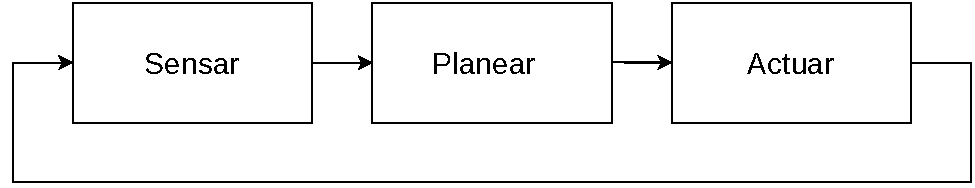
\includegraphics[width=0.8\textwidth]{Figures/Figures_Cap06/hierarchical_paradigm.pdf}
    \caption{Secuencia del Paradigma Jerárquico.}
    \label{fig:hierarchical_paradigm}
\end{figure}

\subsection{Paradigma Reactivo} \label{sub:paradigma_reactivo}

El Paradigma Reactivo surgió a finales de la década de 1980 como solución a problemas que el Paradigma Jerárquico no podía resolver. El modelo reactivo asume que la entrada de una tarea (Actuar) siempre será una salida directa de un sensor (Sensar). Su enfoque fundamental es que todas las acciones del robot son modeladas y realizadas a través de comportamientos. 

Un comportamiento es el conjunto de respuestas que presenta un individuo con relación a su mundo o entorno. Los comportamientos son un mapeo directo de las entradas sensoriales a un patrón de acciones motoras que después se unen para alcanzar una meta. Desde el punto de vista matemático, los comportamientos representan una función de transferencia que transforma entradas sensoriales en comandos de activación \cite{murphy2019introduction}. 

Los sistemas dentro de un paradigma reactivo se componen de comportamientos que mantienen unidos estrechamente la percepción (Sensar) y acción (Actuar), todas las actividades robóticas surgen como resultado de estos comportamientos que operan simultáneamente o en secuencia. La organización de este modelo es Sensar-Actuar sin tomar en cuenta la planificación, la figura  \ref{fig:reactive_paradigm} muestra esto. La percepción en el Paradigma Reactivo es específica o local para comportamiento. Es decir, cada comportamiento tiene acceso directo a uno o más sensores que son independientes de otros comportamientos. En situaciones específicas, más de un comportamiento puede tomar el resultado de un sensor y procesarlo de manera diferente. En esencia, un comportamiento no conoce lo que hace o percibe otro comportamiento. El paradigma reactivo puede combinar comportamientos en una arquitectura mediante dos métodos dominantes: subsunción y suma de campos potenciales.
\begin{figure}
    \centering
    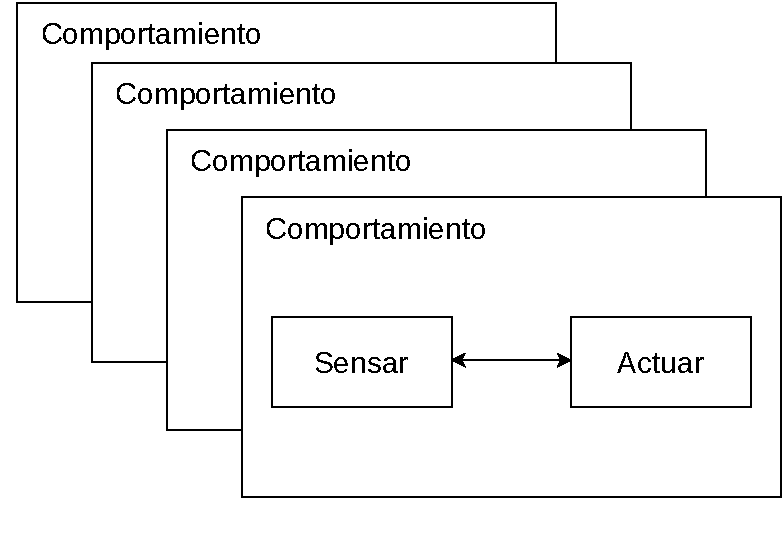
\includegraphics[width=0.5\textwidth]{Figures/Figures_Cap06/reactive_paradigm.pdf}
    \caption{Secuencia del Paradigma Reactivo.}
    \label{fig:reactive_paradigm}
\end{figure}

Las ventajas más reconocidas de este paradigma son los buenos principios de Ingeniería de Software que exhiben los sistemas que lo implementan, los comportamientos se pueden probar de manera independiente. Además, se pueden construir comportamientos más complejos a partir de comportamientos primitivos, existe bajo acoplamiento y alta cohesión. Los comportamientos son inherentemente modulares y fáciles de probar de manera aislada al sistema. Por el contrario, si los comportamientos se implementan de manera deficiente puede derivar en una ejecución lenta. Dentro del paradigma reactivo un robot se vuelve más inteligente mientras más y mejores comportamientos existan. 

Es importante mencionar que el vehículo autónomo de este trabajo toma como base el paradigma reactivo, cada comportamiento que implemente el vehículo debe hacer uso de las herramientas previamente implementadas para efectuar tareas específicas y mientras más comportamientos se definan, el vehículo autónomo tendrá un nivel de independencia más alto.

\subsection{Paradigma Híbrido} \label{sub:paradigma_híbrido}

El paradigma Híbrido o Deliberativo/Reactivo emergió a principios de la década de 1990, es una combinación de muchos de los fundamentos del Paradigma Reactivo y Jerárquico. Bajo las tres primitivas de la robótica, el modelo Deliberativo/Reactivo se puede pensar como Planear y luego Sensar-Actuar (P, S-A), ver figura \ref{fig:hybrid_paradigm}. Donde, la parte de Sensar-Actuar siempre es realizada mediante comportamientos reactivos, mientras que la planificación es resultado de una amplía gama de actividades inteligentes. El término híbrido se da porque la planificación se puede intercalar con la ejecución; luego, en mayor medida, el robot planea un conjunto de comportamientos que más tarde ejecutará por un largo tiempo. La detección también es híbrida; la parte reactiva utiliza representaciones locales en cada comportamiento, mientras que la parte deliberativa usa modelos del mundo global como en el paradigma jerárquico.

Generalmente una arquitectura híbrida tiene los siguientes módulos:
\begin{itemize}
    \item Planificador de misiones
    \item Secuenciador
    \item Administrador de comportamiento
    \item Cartógrafo
    \item Monitor de Rendimiento
\end{itemize}

La regla general para clasificar funciones en deliberativas o reactivas es; funciones que operan con información simbólica forman parte de la capa deliberativa, mientras que las funciones que transforman información de los sensores en comandos de activación van a la capa reactiva. El componente reactivo del modelo está compuesto por comportamientos, por otro lado el deliberativo a menudo se subdivide en capas.
\begin{figure}[h]
    \centering
    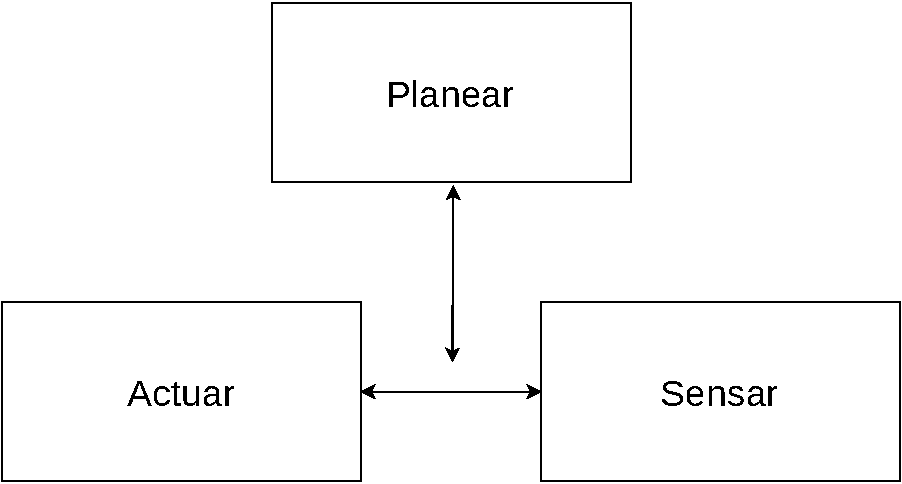
\includegraphics[width=0.5\textwidth]{Figures/Figures_Cap06/hybrid_paradigm.pdf}
    \caption{Secuencia del Paradigma Híbrido.}
    \label{fig:hybrid_paradigm}
\end{figure}

\section{Comportamientos del vehículo} \label{sec:comportamientos_del_vehículo}

\subsection{Crucero} \label{sub:crucero}

De forma similar a como sucede en los sistemas de crucero de un vehículo real, el comportamiento de crucero tiene como objetivo navegar dentro de un circuito vehicular con situaciones controladas y con una velocidad previamente establecida. Estas situaciones incluyen tener un circuito sin obstáculos y mostrar los carriles de la carretera con sus debidas delimitaciones en todo momento, tanto en líneas rectas como en curvas. La figura \ref{fig:cruise_behavior} muestra un escenario con estas condiciones. En otras palabras, el comportamiento de crucero buscar realizar concretamente un seguimiento de carril. Para ello, este comportamiento utiliza el detector y seguidor de carril explicados en el capítulo \ref{cap:seguimiento_de_carriles}, también hace uso de las ecuaciones (\ref{eqn:cruise_speed})-(\ref{eqn:steering_angle}) previamente diseñadas que modelan las leyes de control para las funciones operativas de movimiento lateral y longitudinal respectivamente. Este comportamiento se mantiene activo mientras existan condiciones sin obstáculos en el camino del vehículo.
\begin{figure}[h]
    \centering
    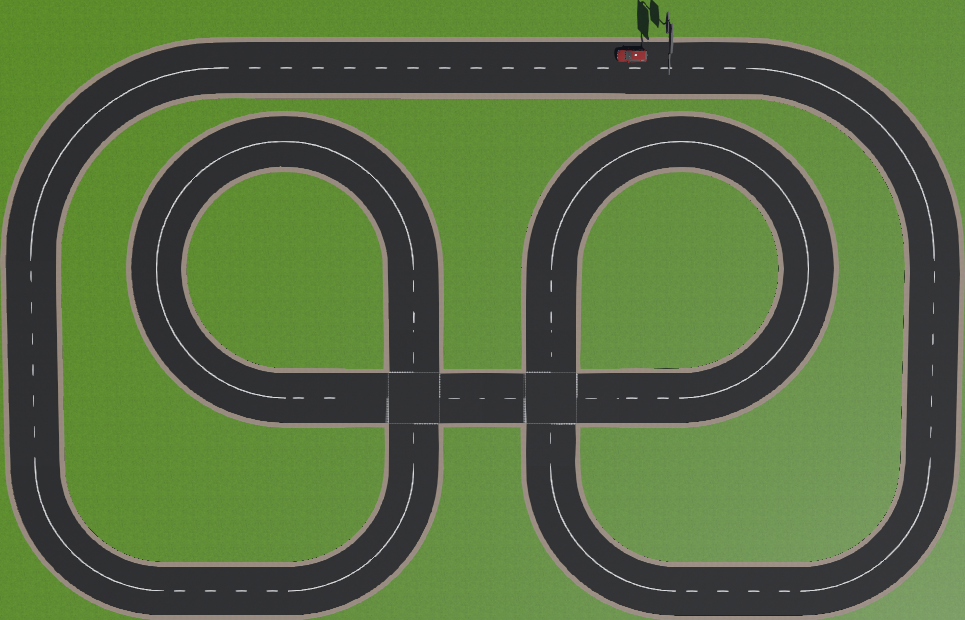
\includegraphics[width=0.5\textwidth]{Figures/Figures_Cap06/crucero.png}
    \caption{Circuito de pruebas sin obstáculos.}
    \label{fig:cruise_behavior}
\end{figure}

\subsection{Mantener distancia} \label{sub:mantener_distancia}

Al incluir vehículos al circuito de pruebas la complejidad en la navegación autónoma aumenta. Este comportamiento como su nombre lo indica pretende mantenerse a distancia con los vehículos presentes en la carretera. El comportamiento de mantener distancia actúa en una situación de tráfico vehicular manteniendo al vehículo autónomo a una distancia segura respecto al vehículo de enfrente para evitar colisiones, ver \ref{fig:keep_distance_behavior}.
%También, se hace uso de la detección y seguimiento de objetos explicados en el capítulo \ref{cap:detección_de_obstáculos}.
Este comportamiento se logra utilizando la detección y seguimiento de carril desarrollados en el capítulo \ref{cap:seguimiento_de_carriles} con una mínima modificación. Primero, la ley de control para el movimiento lateral del vehículo es con la ecuación (\ref{eqn:steering_angle}), que es la misma utilizada para el seguimiento de carril. La diferencia aparece en la ley de control para el movimiento longitudinal, anteriormente se había mencionado que la velocidad del vehículo autónomo sería constante durante todo el recorrido, esto funciona bien para el comportamiento de crucero. Sin embargo, en el caso de seguimiento de vehículos la velocidad debe variar respecto a la distancia del coche de enfrente para no chocar. 
\begin{figure}[h]
    \centering
    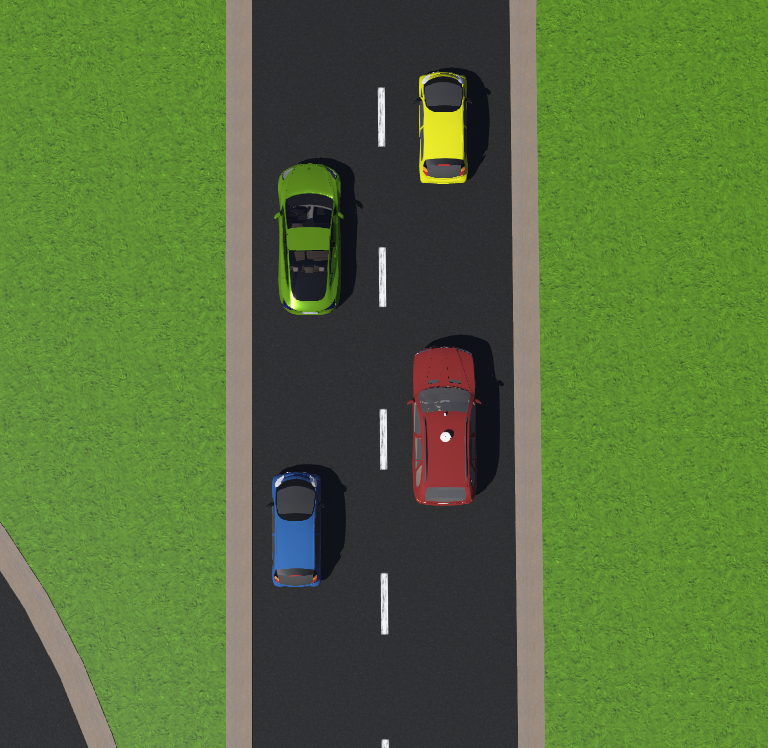
\includegraphics[width=0.5\textwidth]{Figures/Figures_Cap06/keep_distance.png}
    \caption{Ejemplo de posible situación de tráfico.}
    \label{fig:keep_distance_behavior}
\end{figure}

Considerar la figura \ref{fig:safe_distance}, en ella se ilustra una posible situación de tráfico, el vehículo en color rojo es el vehículo autónomo y lo llamaremos $a$, el coche amarillo lo nombraremos $b$. Es evidente que en está situación no se puede manejar libremente solo siguiendo las líneas del carril con velocidad constante. Por ello en este comportamiento cuando el vehículo $b$ se encuentre a una distancia muy cercana con $a$ se debe de disminuir la velocidad de $a$, cuando el vehículo $b$ esté más lejos, la velocidad de $a$ aumenta. Es decir, el coche $a$ aumenta o disminuye su velocidad proporcionalmente a la distancia $d$. Con esta proporción entre velocidad y distancia se logra seguir al vehículo del frente a una distancia segura y evitar colisiones, por otro lado, las colisiones en los laterales se evitan con el seguimiento de carril, pues la ley de control del movimiento lateral mantiene al vehículo autónomo dentro de su carril.
\begin{figure}[h]
    \centering
    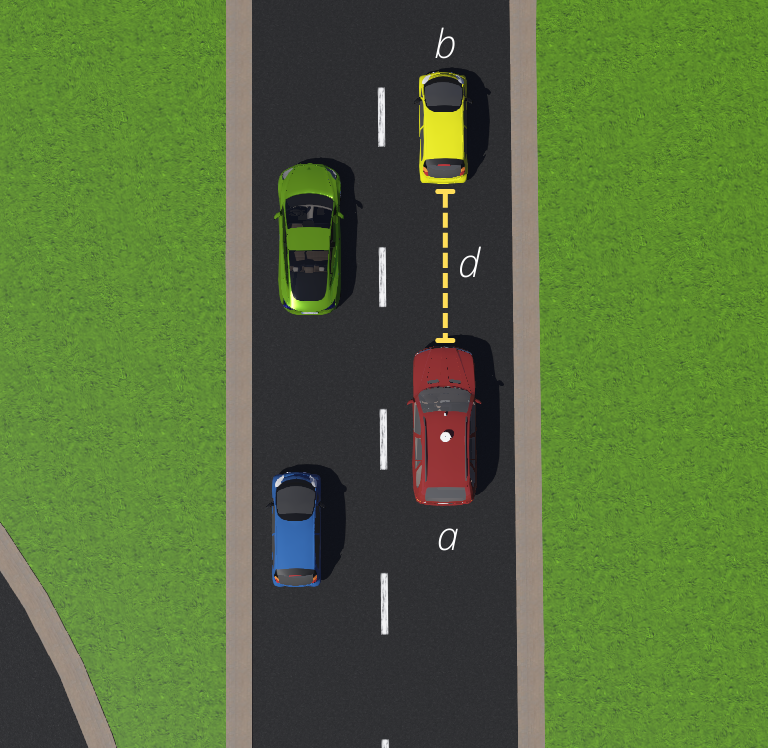
\includegraphics[width=0.5\textwidth]{Figures/Figures_Cap06/safe_distance.png}
    \caption{Distancia Segura, $d(a, b)$.}
    \label{fig:safe_distance}
\end{figure}

La distancia $d$ que existe entre el vehículo autónomo y el vehículo de enfrente la llamaremos ``distancia segura'', ver \ref{fig:safe_distance}. Con esta distancia se calcula la velocidad del vehículo autónomo. Entonces, para este comportamiento la ecuación (\ref{eqn:cruise_speed}) que representa la ley de control de movimiento longitudinal se expresa de la siguiente forma:
\begin{equation}
    v = d * k
    \label{eqn:keep_distance_velocity}
\end{equation}
donde, $d$ es la distancia entre $a$ y $b$, mientras que $k$ es una constante de proporcionalidad para aumentar o disminuir velocidad. El comportamiento mantener distancia entra en acción cuando se presentan situaciones donde no es posible mantenerse en crucero o cuando no se pueda realizar un rebase.

\subsection{Rebase} \label{sub:rebase}

El rebase es un comportamiento especial porque cambia considerablemente las leyes de control previamente establecidas para el movimiento lateral y longitudinal. Un rebase requiere de diferentes acciones que involucran el cambio de dirección en las llantas y mantener la velocidad en un rango aceptable, estas acciones deben de ser bien planeadas para evitar choques con el vehículo por rebasar.

Para implementar un comportamiento de rebase en este trabajo específico se optó por realizarlo en condiciones de lazo abierto, es decir, no existe ningún tipo de retroalimentación como en los comportamientos de crucero y seguimiento de vehículos donde la retroalimentación al sistema provenía del error en los carriles detectados y la distancia segura respectivamente. Se entiende que bajo las normas de conducción vehicular solo se pueden efectuar rebases por el carril izquierdo. Por lo tanto, una vez que se detecta una posible situación de rebase se ejecuta una máquina de estados específica que cumple con esta acción, ver figura \ref{fig:pass}. A continuación se enuncia la secuencia de pasos a seguir para realizar un rebase:
\begin{enumerate}
    \item Girar a la izquierda $t$ segundos.
    \item Girar a la derecha $t/2$ segundos para alinear.
    \item Avanzar en línea recta $t$ segundos.
    \item Girar a la derecha $t$ segundos.
    \item Girar a la izquierda $t/2$ segundos para alinear.
    \item Avanzar en línea recta $t$ segundos.
\end{enumerate}
\begin{figure}[h]
    \centering
    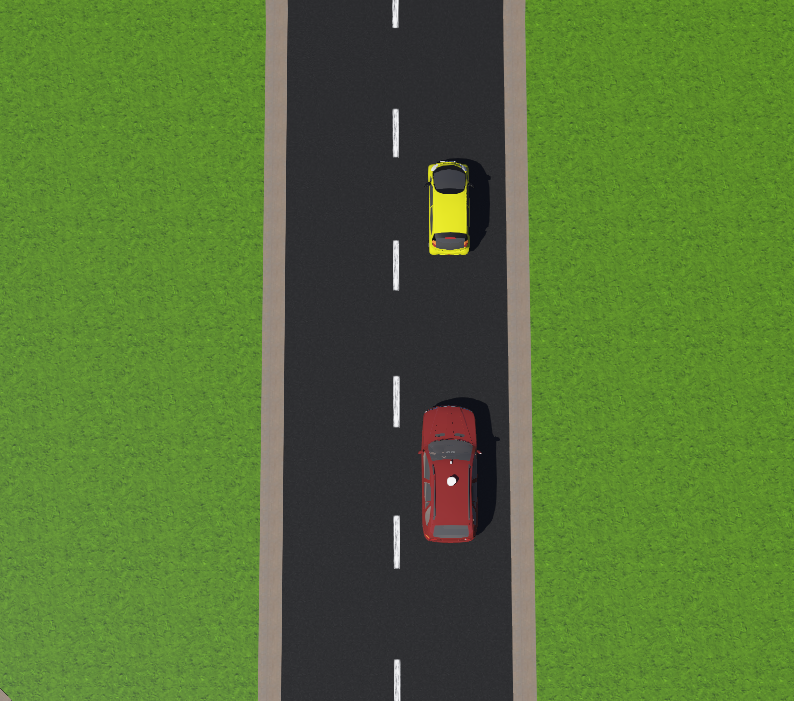
\includegraphics[width=0.5\textwidth]{Figures/Figures_Cap06/rebase.png}
    \caption{Situación de rebase.}
    \label{fig:pass}
\end{figure}


Una vez conocidos estos pasos es fácil diseñar una máquina de estados para rebase, la figura \ref{fig:pass_sm} representa la carta ASM para esta máquina de estados.

Durante el rebase se considera una velocidad constante pero menor a la velocidad utilizada en el seguimiento de carril.
\begin{equation}
    v_r < v
\end{equation}
Para controlar el \textit{steering} del vehículo en giros a la izquierda el ángulo de dirección es $\delta < 0$ y en giros a la derecha $\delta > 0$. Además, se toma en cuenta el ángulo de dirección actual del vehículo, de esto modo la ecuación (\ref{eqn:steering_angle}) para movimiento lateral se transforma en:
\begin{equation}
    \delta = \delta_{actual} + \theta
    \label{eqn:right_steering}
\end{equation}
para giros a la derecha, y
\begin{equation}
    \delta = \delta_{actual} - \theta
    \label{eqn:left_steering}
\end{equation}
para giros a la izquierda.
\begin{figure}[h]
    \centering
    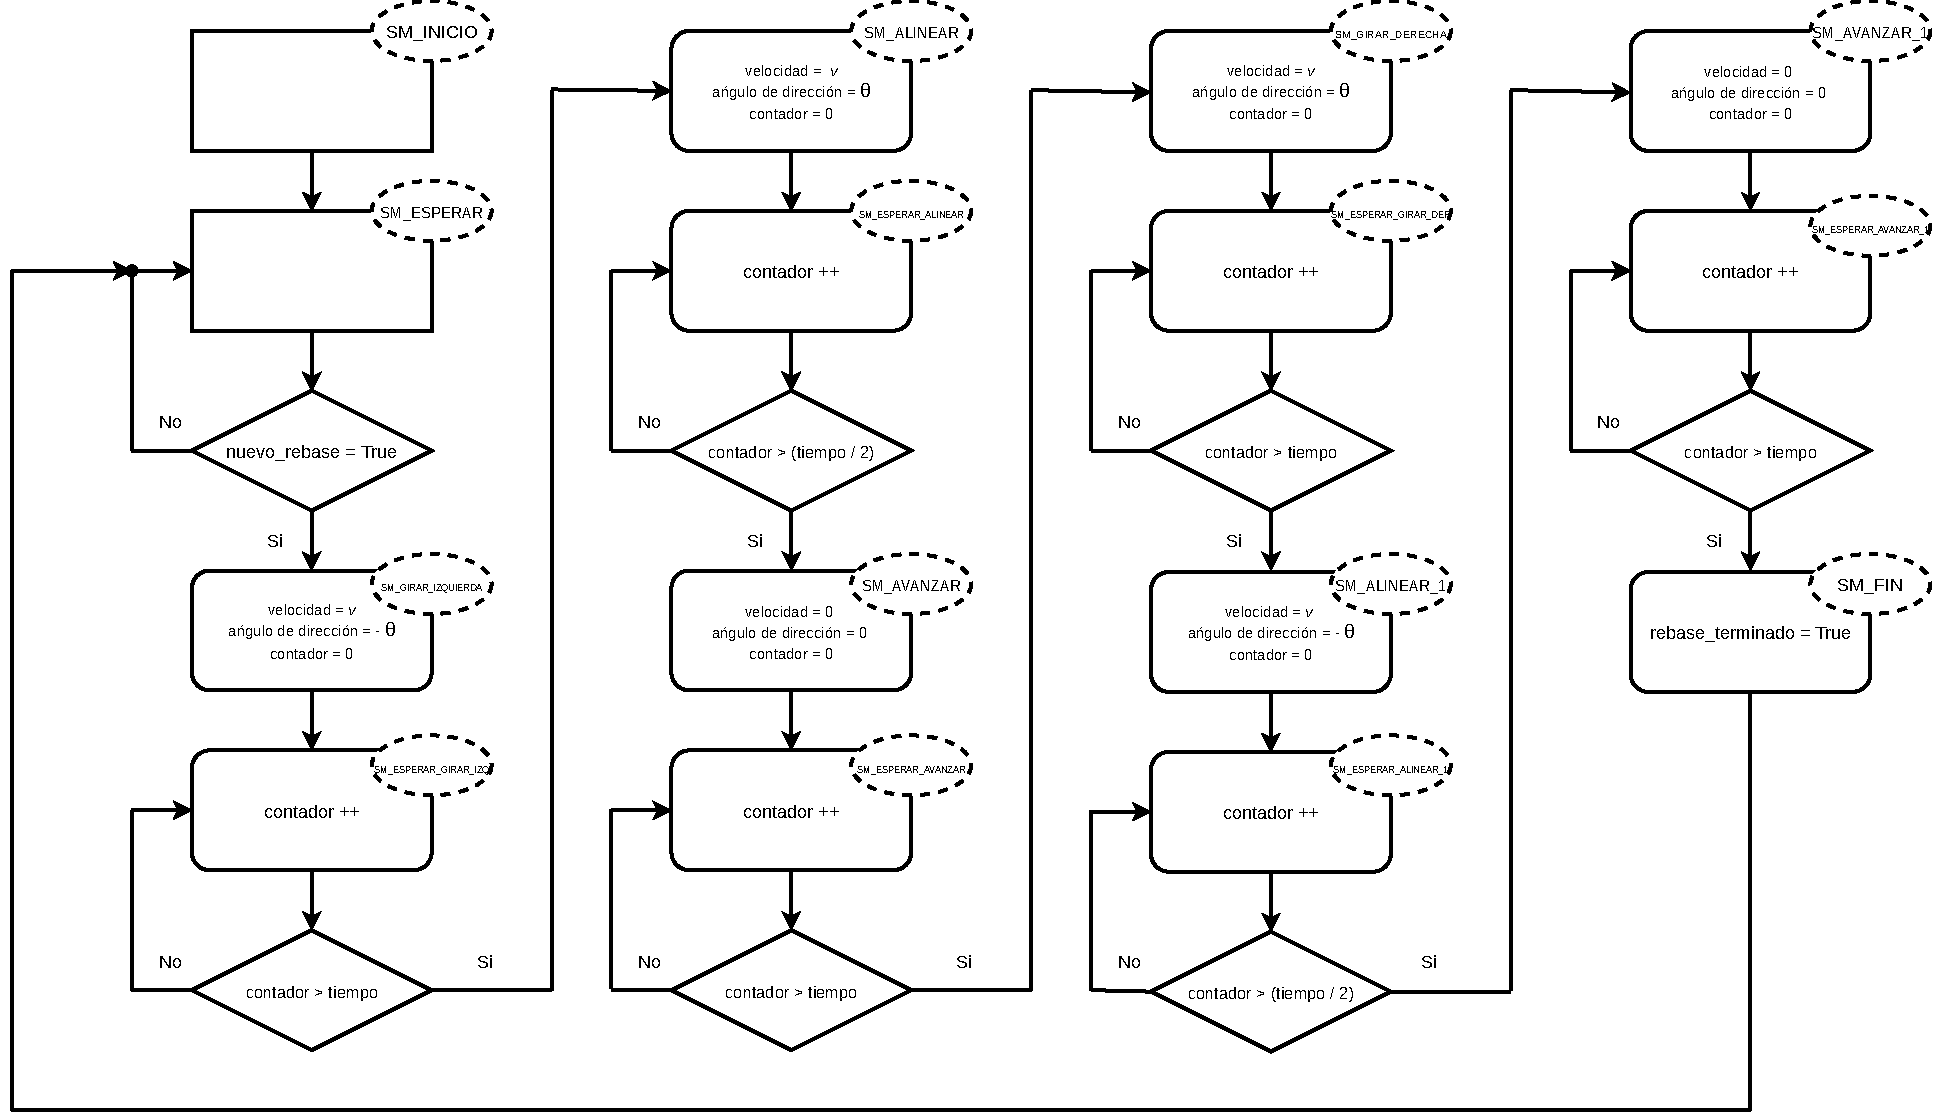
\includegraphics[width=1.0\textwidth]{Figures/Figures_Cap06/sm_pass.pdf}
    \caption{Máquina de estados para acción de rebase.}
    \label{fig:pass_sm}
\end{figure}

En las ecuaciones (\ref{eqn:right_steering})-(\ref{eqn:left_steering}), $\theta$ representa un ángulo constante para provocar un giro a la izquierda o a la derecha según corresponda. Esta constante $\theta$ como el tiempo $t$ fueron obtenidos mediante experimentación del comportamiento de rebase. El resultado esperado al implementar la carta ASM de la figura \ref{fig:pass_sm} es el que se muestra en \ref{fig:pass_behavior}, donde se observa la secuencia de pasos que debe de seguir el vehículo autónomo para lograr un rebase seguro. El comportamiento de rebase se activa siempre y cuando existan condiciones seguras para evitar choques, es decir, que no existan vehículos cercanos al frente, por detrás y al costado izquierdo del vehículo. También, se considera que lo más seguro después de completar un rebase es volver al comportamiento de crucero.

\begin{figure}[h]
    \centering
    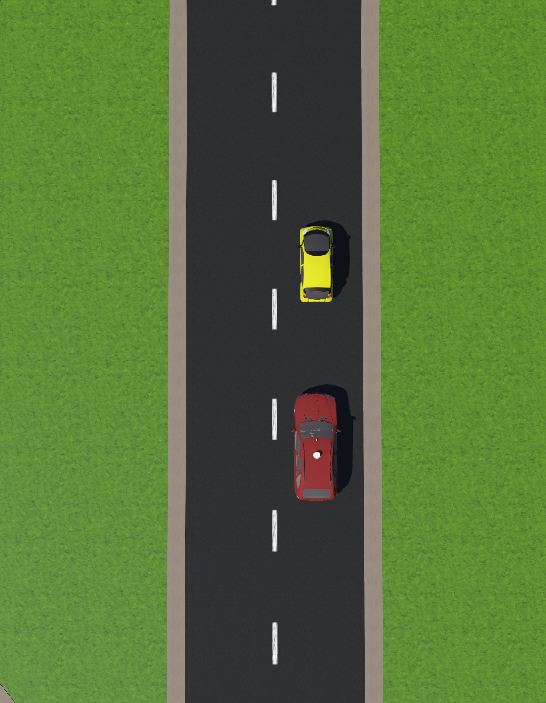
\includegraphics[width=0.15\textwidth]{Figures/Figures_Cap06/pass_1.png}
    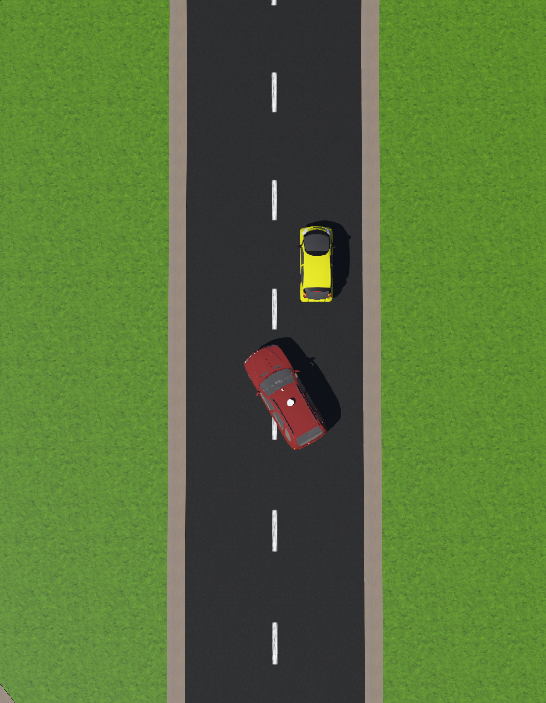
\includegraphics[width=0.15\textwidth]{Figures/Figures_Cap06/pass_2.png}
    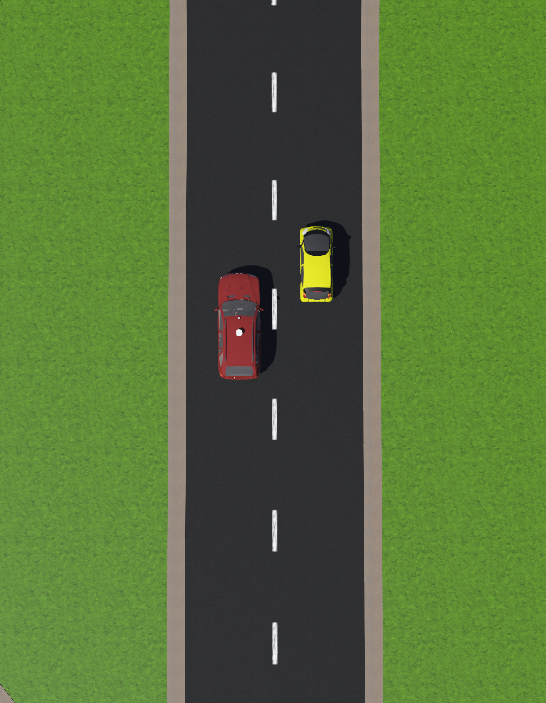
\includegraphics[width=0.15\textwidth]{Figures/Figures_Cap06/pass_3.png}
    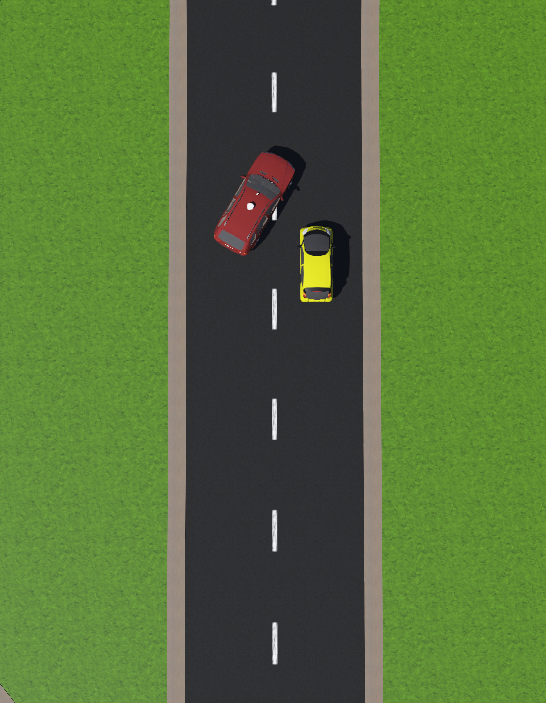
\includegraphics[width=0.15\textwidth]{Figures/Figures_Cap06/pass_4.png}
    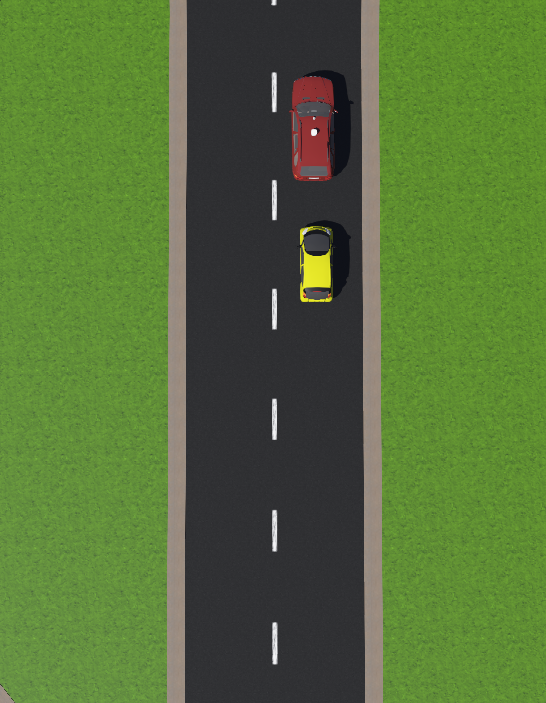
\includegraphics[width=0.15\textwidth]{Figures/Figures_Cap06/pass_5.png}
    \caption{Secuencia para comportamiento de rebase.}
    \label{fig:pass_behavior}
\end{figure}

\subsection{Árbitro} \label{sub:árbitro}

El árbitro es un sistema que permite tomar decisiones y cambiar al comportamiento más adecuado en cada situación que se presente durante la navegación autónoma en el circuito. Para elegir entre los comportamientos crucero, mantener distancia y rebase, el árbitro percibe el ambiente del vehículo en todo momento. Mientras el vehículo avanza se ejecuta el algoritmo de agrupación \textit{k-means} de la sección \ref{sub:ejemplo_de_implementación_del_algoritmo_K-medias}, posteriormente el EKF diseñado en \ref{sub:estimación_de_posición_y_velocidad_con_el_filtro_de_kalman_extendido} estima la posición y velocidad de los obstáculos (vehículos) detectados. Con base en estas mediciones el árbitro es capaz de definir diferentes escenarios y elegir el comportamiento que mejor se acople.

Dentro del circuito es posible que existan múltiples vehículos en diferentes posiciones, sin embargo, para este proyecto se toman en cuenta cuatro posibles obstáculos que influyan en el cambio de comportamiento del vehículo. Considerar la figura \ref{fig:obstacle_zones}, en ella se muestra el vehículo de pruebas en color rojo y los objetos en color amarillo son las posibles posiciones de los vehículos obstáculo. Las etiquetas de los vehículos amarillos corresponden a la zona donde se encuentran, para estas zonas se considera al vehículo autónomo (rojo) como el punto de origen,  las zonas son:
\begin{enumerate}
    \item Norte (N)
    \item Este  (E)
    \item Noroeste (NE)
    \item Suroeste (SE)
\end{enumerate}

\begin{figure}[h]
    \centering
    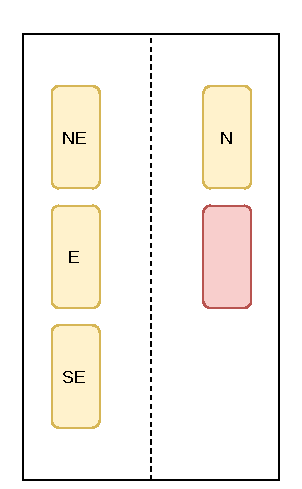
\includegraphics[width=0.25\textwidth]{Figures/Figures_Cap06/zones.pdf}
    \caption{Zonas de obstáculos.}
    \label{fig:obstacle_zones}
\end{figure}

Teniendo en cuenta esta configuración de zonas es claro que un vehículo puede o no ocupar una zona, al considerar cuatro posibles vehículos como obstáculos se pueden presentar $4^2 = 16$ estados posibles. Cada uno de estos estados se aprecian abiertamente en la figura \ref{fig:states}, donde 0 representa una zona ocupada y 1 para zona libre.
\newpage
\begin{figure}[h]
    \centering
    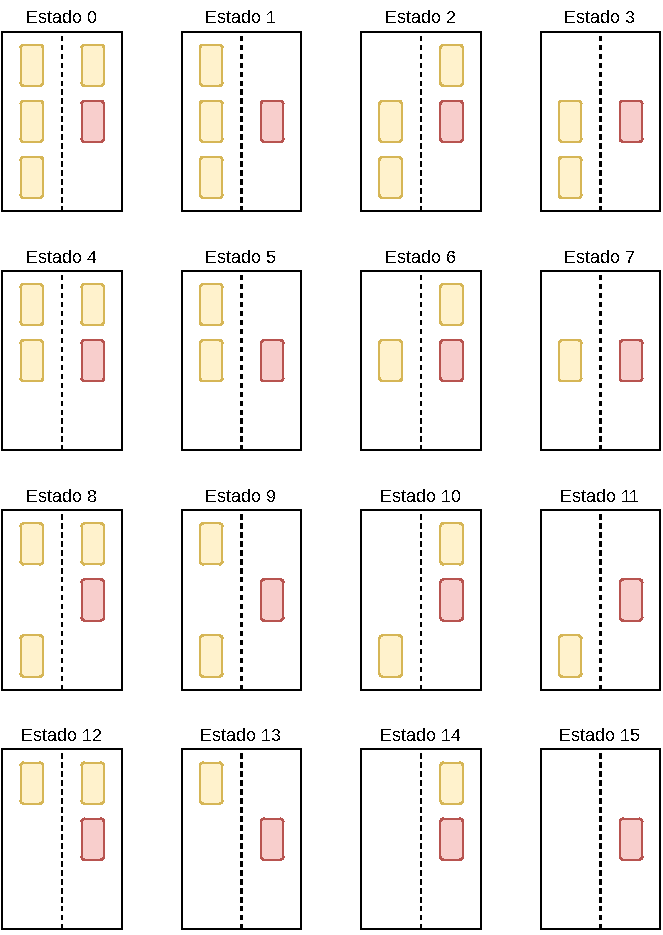
\includegraphics[width=0.75\textwidth]{Figures/Figures_Cap06/states.pdf}
    \caption{Estados considerados.}
    \label{fig:states}
\end{figure}

\newpage
La información de los posibles estados de la figura \ref{fig:states} se puede ver en forma tabular. A continuación, el cuadro \ref{tab:states} indica cual es el comportamiento más adecuado para cada estado.
\begin{table}[h]
    \begin{center}
        \begin{tabular}{cccc||l}
        \hline
            E & SE & NE & N & Comportamiento\\ \hline \hline
            0 & 0 & 0 & 0 & Mantener Distancia\\ 
            0 & 0 & 0 & 1 & Crucero\\
            0 & 0 & 1 & 0 & Mantener Distancia\\
            0 & 0 & 1 & 1 & Crucero\\
            0 & 1 & 0 & 0 & Mantener Distancia\\
            0 & 1 & 0 & 1 & Crucero\\
            0 & 1 & 1 & 0 & Mantener Distancia\\
            0 & 1 & 1 & 1 & Crucero\\
            1 & 0 & 0 & 0 & Mantener Distancia\\
            1 & 0 & 0 & 1 & Crucero\\
            1 & 0 & 1 & 0 & Rebase\\
            1 & 0 & 1 & 1 & Crucero\\
            1 & 1 & 0 & 0 & Mantener Distancia\\
            1 & 1 & 0 & 1 & Crucero\\
            1 & 1 & 1 & 0 & Rebase\\
            1 & 1 & 1 & 1 & Crucero\\ \hline
        \end{tabular}
    \end{center}
    \caption{Tabla de estados.}
    \label{tab:states}
\end{table}

Con la tabla anterior se puede notar que en 6 de los 16 estados ($37.5\%$) el comportamiento más adecuado es mantener distancia, en 8 ocasiones ($50.0\%$) lo más apropiado es la conducción mediante el comportamiento de crucero y solo en 2 de los 16 estados ($12.5\%$) existen condiciones seguras para realizar un rebase de vehículo. 

De forma similar a la implementación del comportamiento de rebase, el árbitro también hace uso de una máquina de estados donde se incluyen todas las condiciones vistas en la tabla \ref{tab:states} para escoger el comportamiento apropiado. La carta ASM que representa a la máquina de estados del árbitro se puede ver en \ref{fig:main_sm}.
\begin{figure}[h]
    \centering
    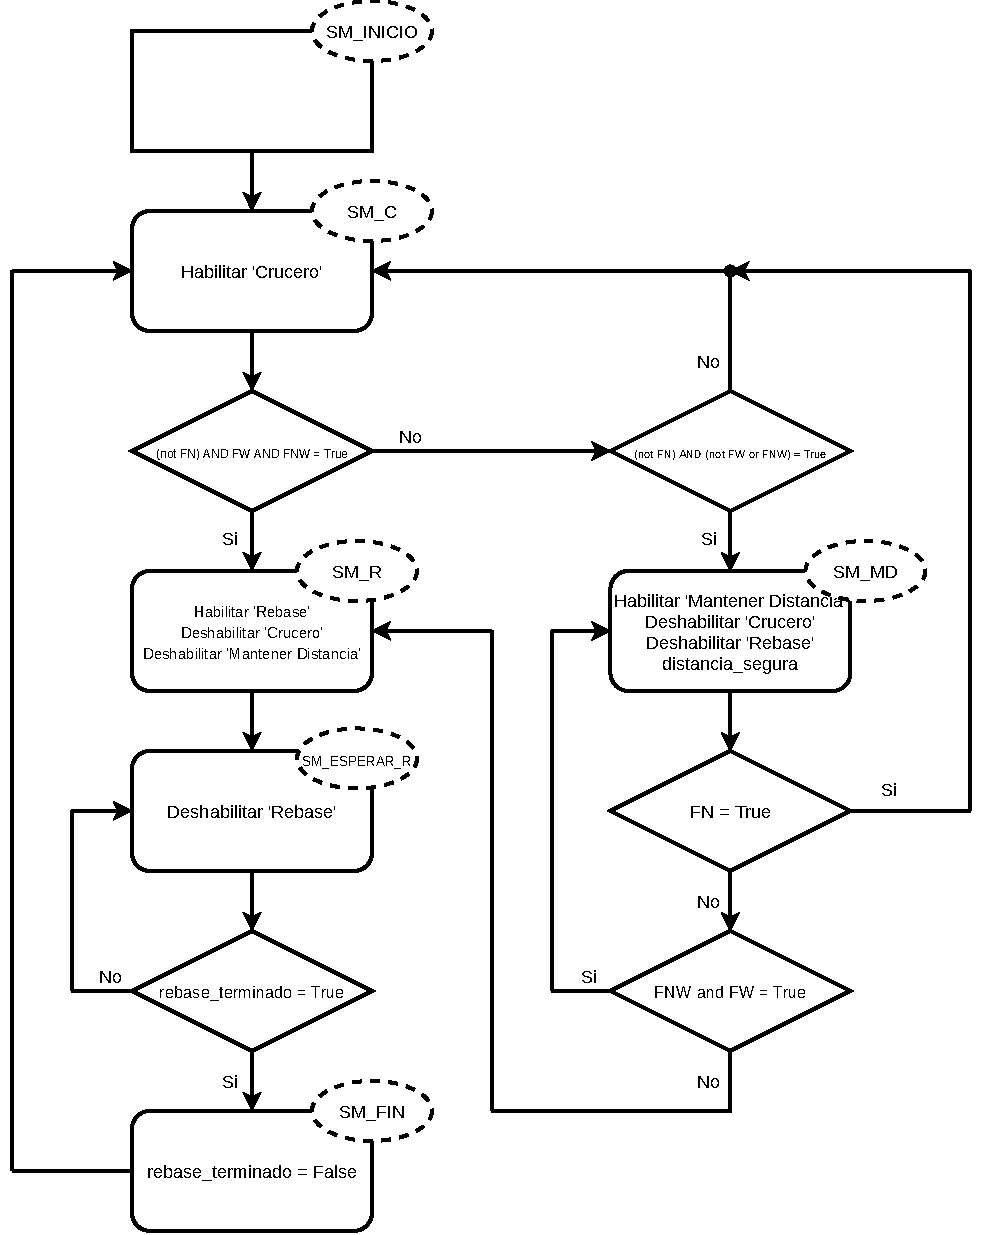
\includegraphics[width=0.7\textwidth]{Figures/Figures_Cap06/main_sm.pdf}
    \caption{Máquina de estados para decidir comportamiento.}
    \label{fig:main_sm}
\end{figure}

Mediante esta máquina de estados el árbitro puede habilitar y deshabilitar comportamientos según sea necesario, además puede enviar y recibir las variables de ``distancia segura'' y ``rebase terminado'' para el control de los comportamientos de mantener distancia y rebase respectivamente. 

Al concluir este capítulo se definieron los comportamientos con los que contará el vehículo autónomo, cada uno de ellos es utilizado en situaciones y tareas específicas. También, se mencionó que un árbitro estará a cargo de la elección. Es posible que el árbitro sea la parte más importante del sistema de navegación del vehículo autónomo porque es el encargado de decidir el comportamiento adecuado a cada situación, de modo que, si llega a fallar en la elección puede tener como consecuencia salir del camino o en un caso más extremo chocar con algún vehículo. Con estas nuevas características, el sistema de navegación del vehículo autónomo es mucho más completo y ahora debe ser capaz de conducir de forma autónoma en espacios supervisados. 

En el capítulo siguiente se expondrán diferentes retos de navegación para el vehículo autónomo donde se pondrán a prueba todos los módulos diseñados e implementados como el detector y seguidor de carril, el sistema para detección y seguimiento de objetos, así como el árbitro que deberá seleccionar el comportamiento apropiado en cada situación como ya se ha mencionado reiteradamente.

